%-------------------------------------------------------------------------------
%	EIC CHAPTER
%-------------------------------------------------------------------------------
\label{ch:eic}
It has been known for nearly a century that atoms are composed of nucleons (protons and neutrons), but it took another 50 years for Murray Gell-Mann and George Zweig to independently develop a model proposing that nucleons themselves are made up of constituent components, called quarks, bound together by the exchange of gluons \cite{SLACquark}. This lead to the development of the fundamental theory of the strong interaction, known as Quantum Chromo-Dynamics (QCD). It is now a strong goal of the nuclear physics community to understand the interactions of quarks and gluons and how those interactions make manifest both nucleons themselves, which account for nearly all the mass of the visible matter in the universe, as well as the nucleons' spin, mass, and magnetic moment.

Although it would theoretically be possible to study these properties using fixed-target electron beam experiments, it is three-fold prohibitive: it is much more costly to construct an accelerator to accelerate electrons to the necessary momentum (on the order of TeV) than to build a collider, it is more difficult and complicated to do transverse nucleon polarization studies with a fixed target due to the nature of the magnetic fields required, and it is very difficult to study the beam fragments of a fixed target reactions due to final state interactions whereas in a collider the fragments will be boosted in the same direction as the beam \cite{Frankfurt} \comment{is this the correct citation to use??}. It was therefore deemed a priority by the 2007 Nuclear Science Advisory Committee's Long-Range Plan that an Electron-Ion Collider (EIC) be the next facility to be built in the United States.

%-------------------------------------------------------------------------------
%	SCIENCE GOALS SECTION
%-------------------------------------------------------------------------------
\section{Science Goals}
One major question still pestering nuclear physicists is "What is the origin of the nucleon spin?". In the 1980s the naive answer was that the total nucleon spin was the sum of the spin of its three valance quarks, but many years of experimentation has revealed that it is much more complicated (Fig. \ref{fig:nucleon_spin}). The EIC will be capable of much more detailed study of the contributions to the nucleon structure by enabling multi-dimensional projections of the distribution of quarks and gluons in space, longitudinal and transverse momenta, spin, and flavor.

\begin{figure}[ht]
	\centering
	\includegraphics[scale=.08]{nucleon_spin.png}
	\caption{Evolution of our understanding of nucleon spin structure. \textbf{Left:} In the 1980s, a nucleon’s spin was naively explained by the alignment of the spins of its constituent quarks. \textbf{Right:} In the current picture, valence quarks, sea quarks and gluons, and their possible orbital motion are expected to contribute to overall nucleon spin. Figure from reference \cite{EICWhitePaper}}
	\label{fig:nucleon_spin}
\end{figure}

\subsection{Nucleon Spin}
\comment{maybe these are unnecessary subsections? Could probably just expand on the science goals section a little more}
\subsection{Quark/Gluon Distribution}

%-------------------------------------------------------------------------------
%	FACILITIES SECTION
%-------------------------------------------------------------------------------
\section{Facilities}
As of the writing of this thesis there are two competing deigns for an EIC facility to be built in the United States: a figure-8 accelerator design for Thomas Jefferson National Accelerator Facility (JLab) (Figure \ref{fig:jleic_layout}), and a ring-ring accelerator design for Brookhaven National Lab (BNL) (Figure \ref{fig:erhic_layout}).

\begin{figure}[ht]
	\centering
	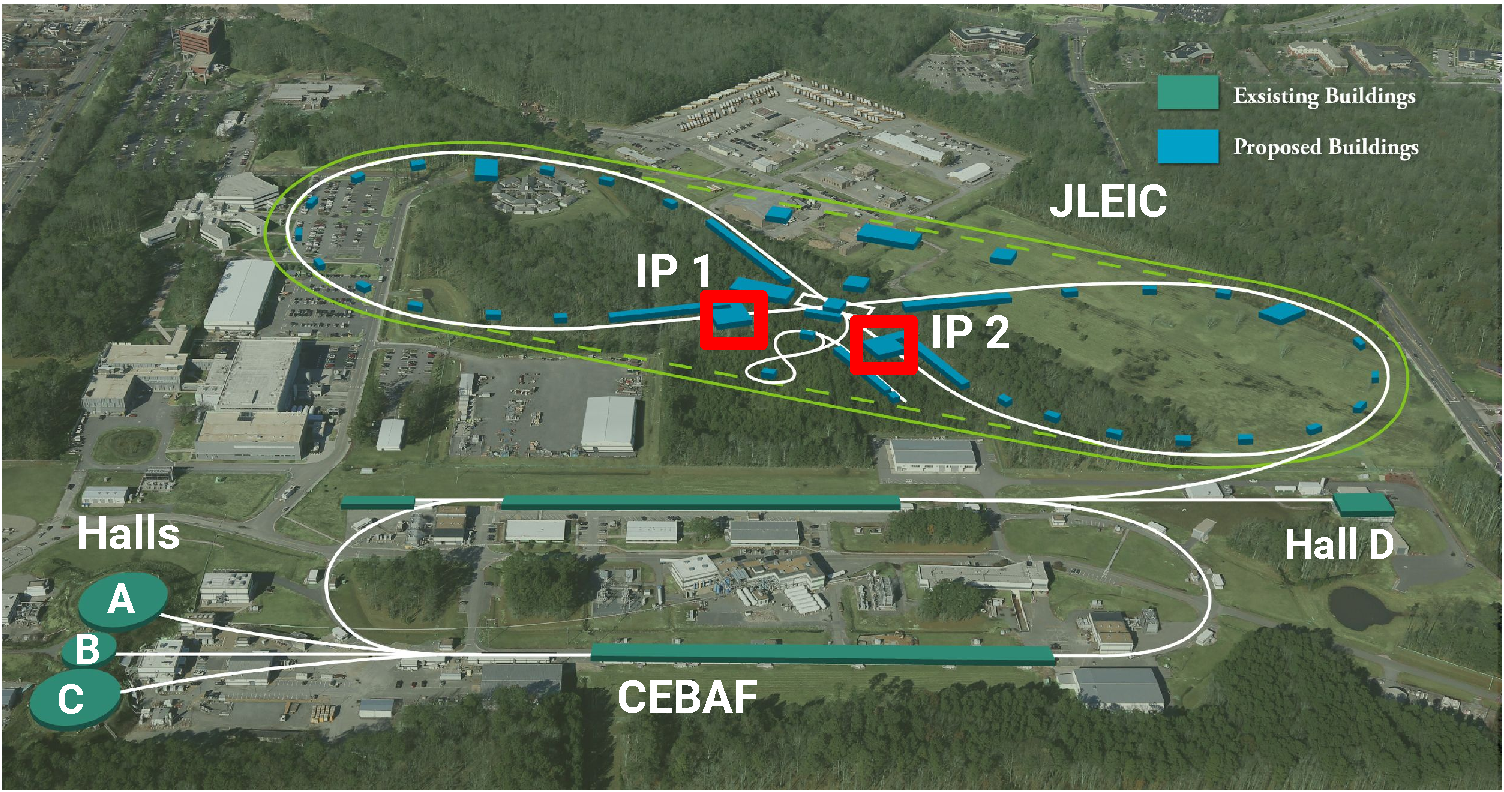
\includegraphics[scale=0.5]{JLEIC_layout2.pdf}
	\caption{Current design of the EIC facility for JLab with the two interaction points highlighted in red.}
	\label{fig:jleic_layout}
\end{figure}

\begin{figure}[ht]
	\centering
	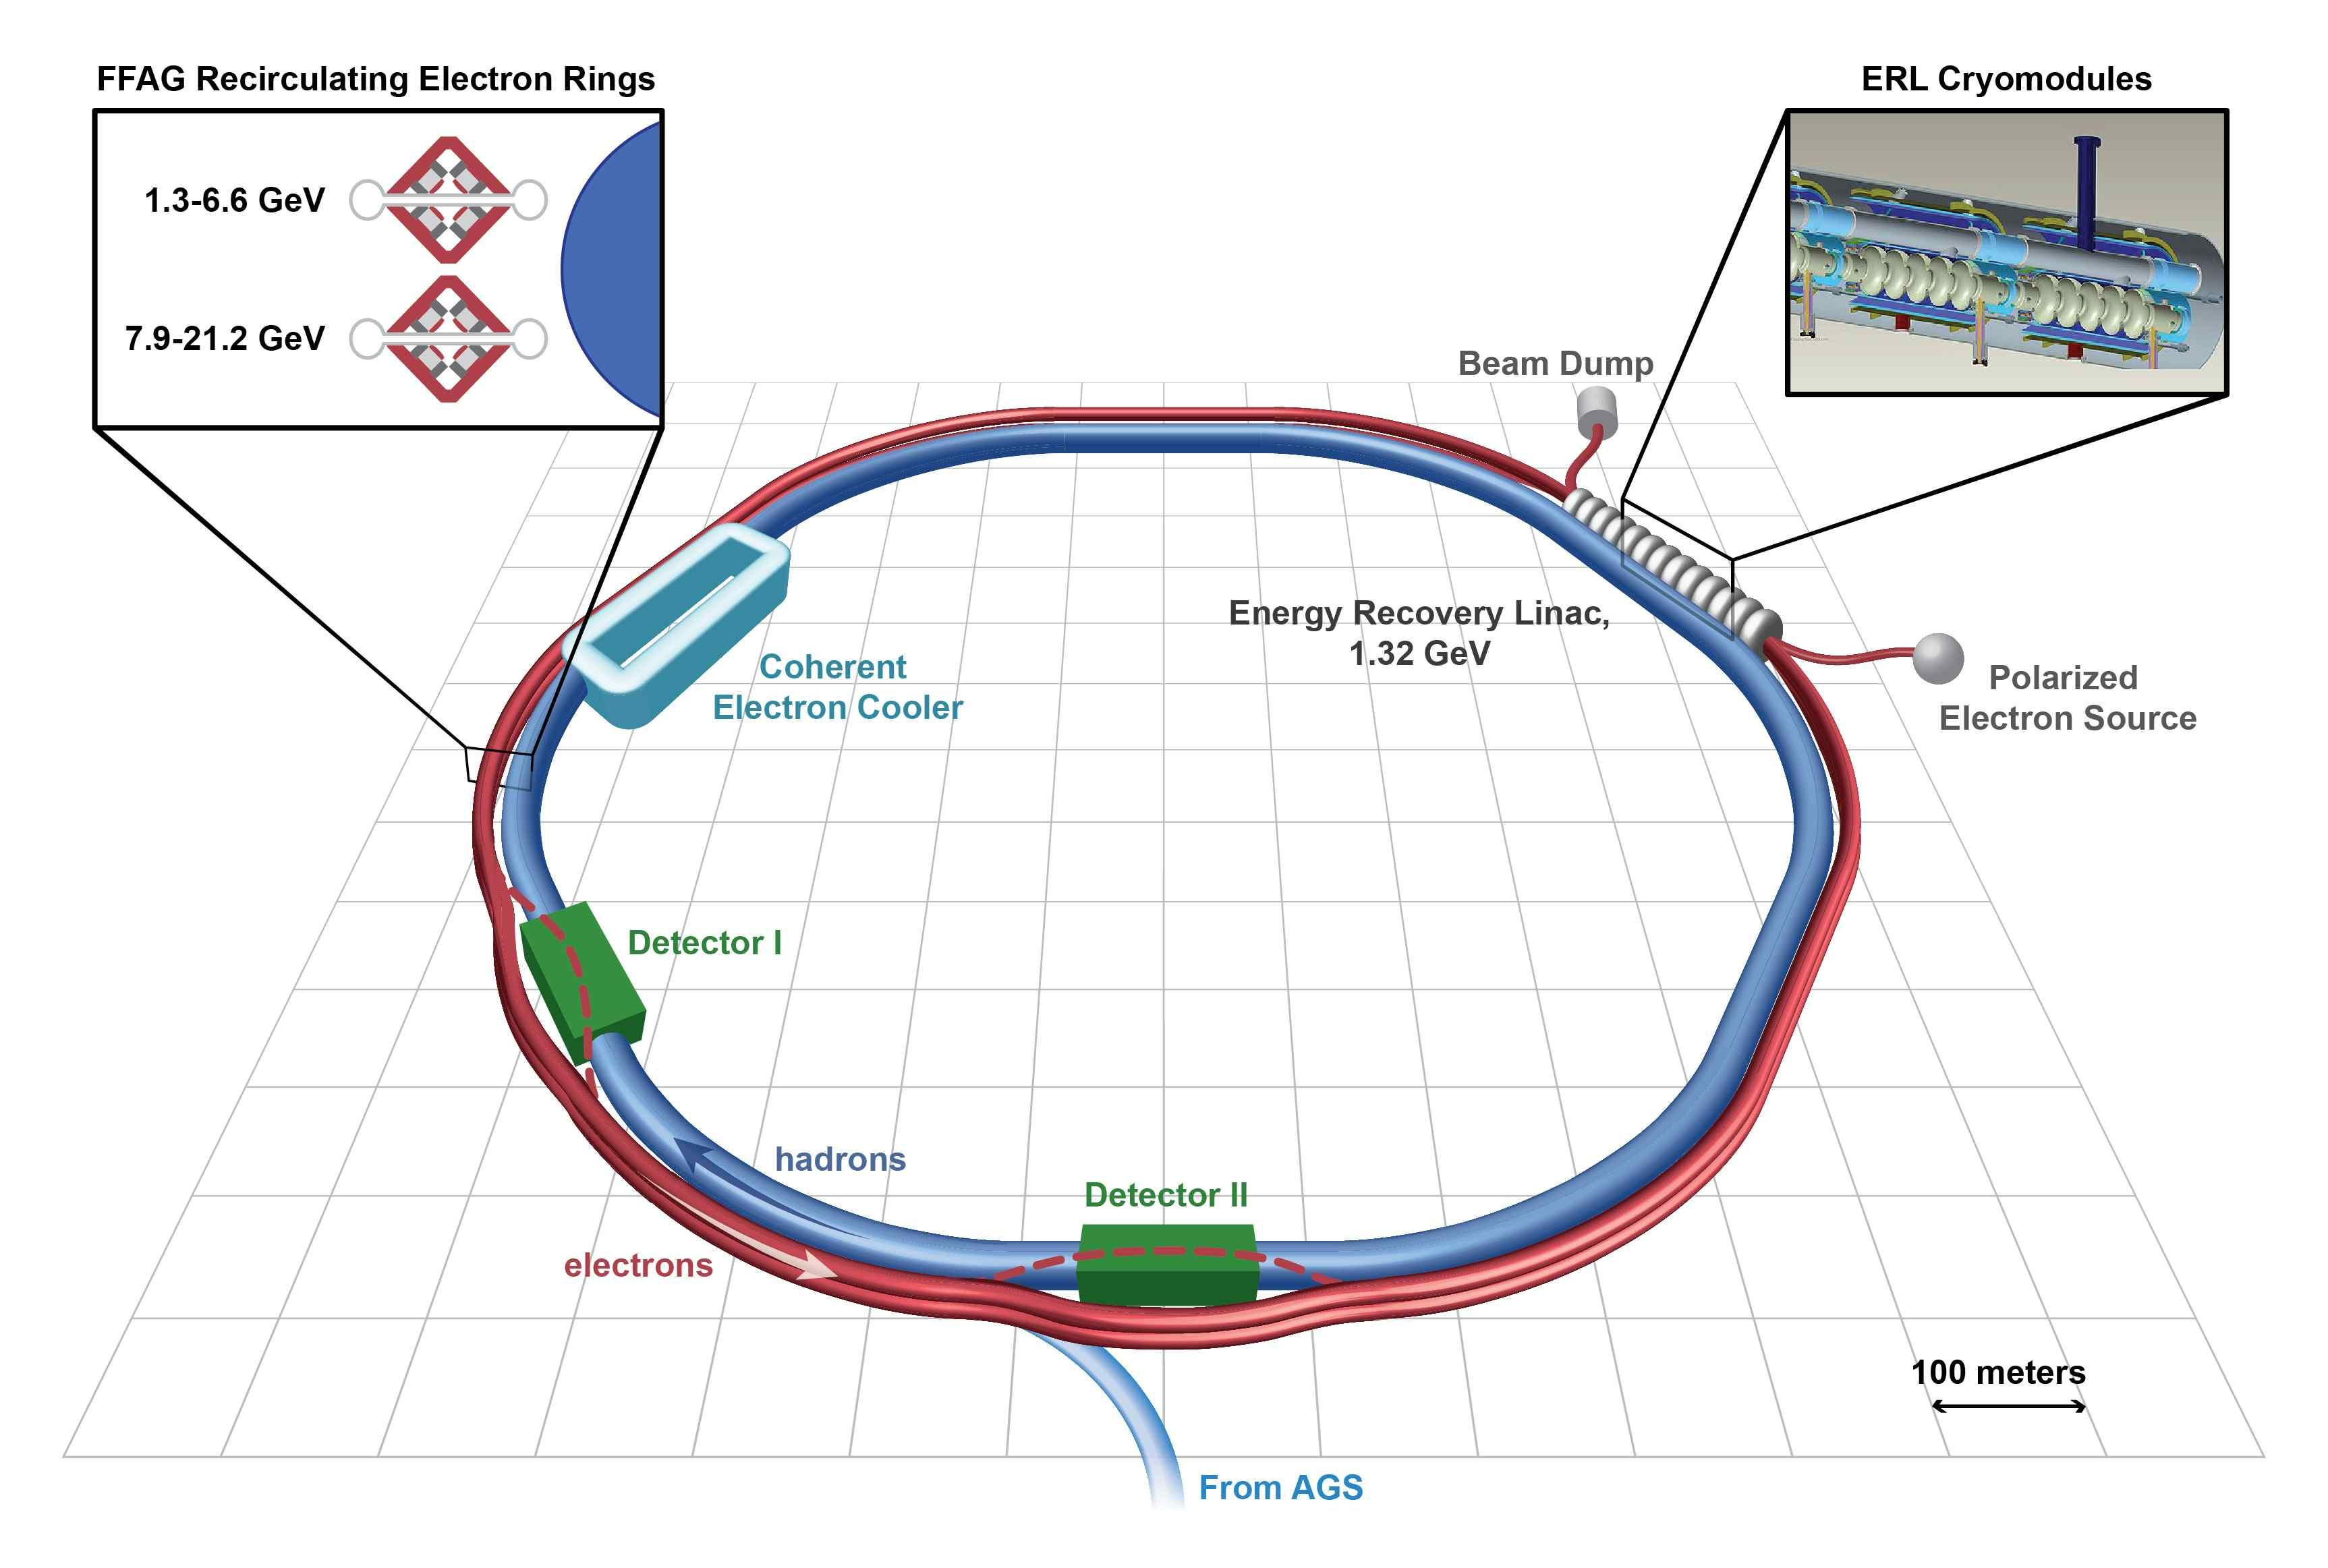
\includegraphics[scale=0.12]{eRHIC_Layout.jpeg}
	\caption{Current design of the EIC facility for BNL.}
	\label{fig:erhic_layout}
\end{figure}

The JLab EIC (JLEIC) is planned to be approximately 1.4 km in circumference and have a footprint of roughly 500 m by 170 m. The design is a ring-ring with electrons and ions being stored in separate beam lines and collided at two interaction points  (IPs) (outlined in red in Figure \ref{fig:jleic_layout}) on the figure-8. The JLab CEBAF SRF linac will be used as an electron injector for electrons with 3 - 11 GeV energy. The second ring will store an ion beam with energy of 20 to 100 GeV for protons or up to 40 GeV per nucleon for light to heavy ions. The ion beams are generated and accelerated in a new ion injector complex with the same figure-8 design that will be utilized to preserve ion polarization. The two rings will be stacked vertically in the same underground tunnel \cite{JLEICdesign}.

The BNL facility, named eRHIC, will use a new electron beam facility based on an Energy Recovery LINAC that will be built inside of the Relativistic Heavy Ion Collider (RHIC) tunnel to collide with RHIC's pre-existing polarized proton/ion beam (Fig. \ref{fig:erhic_layout}). \comment{I feel like I should say more about eRHIC here since I said so much about JLEIC}

%-------------------------------------------------------------------------------
%	JLEIC DETECTOR SECTION
%-------------------------------------------------------------------------------
\subsection{JLEIC Detector Design}
The large center of mass energies of reactions at an EIC necessitate a very sophisticated detector system. Figure \ref{fig:jleic_detector} shows the current design of the JLab EIC detector at IP1. This 

\begin{figure}
	\centering
	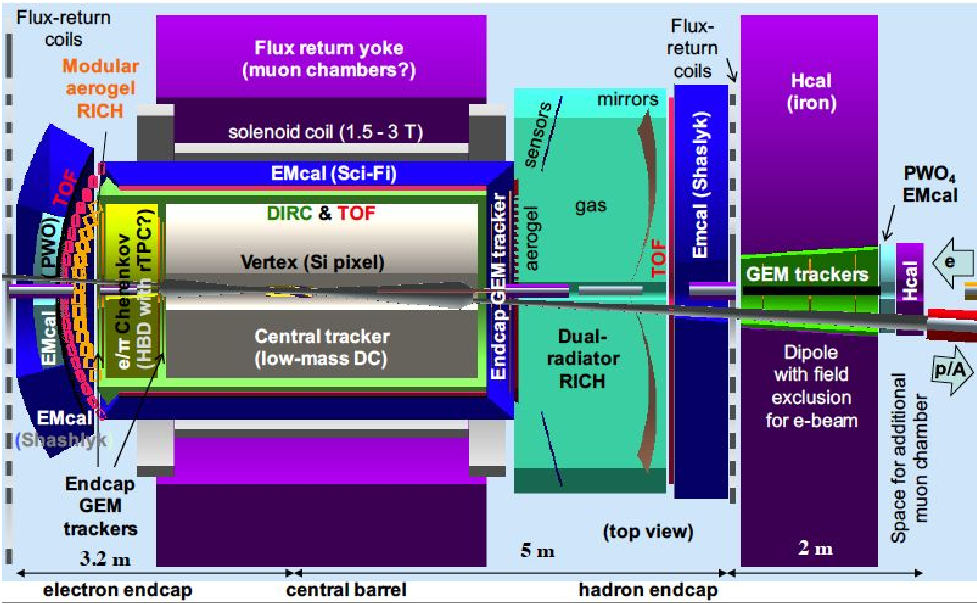
\includegraphics[scale=1]{JLEIC_detector.pdf}
	\caption{Current design of the detector to be used in the JLab EIC at IP1}
	\label{fig:jleic_detector}
\end{figure}

%-------------------------------------------------------------------------------
%	PARTICLE ID SUBSECTION
%-------------------------------------------------------------------------------
\subsection{Particle Identification}
The ability to accurately identify hadrons in the final state is a key requirement for the physics program at an EIC.